% !TeX root=maintext.tex
% !TeX TS-program = XeLaTeX
% !TEX spellcheck = fa
% chapter2

\chapter{ادبیات موضوع}\label{chapter:2}
\thispagestyle{empty}
\epigraph{
«هر نادانی می‌تواند کدی بنویسد که کامپیوتر بفهمد. برنامه‌نویسان خوب کدی می‌نویسند که انسان‌ها می‌توانند آن را بفهمند!»
}
{$ \maltese $ {\large مارتین فاولر}}
\noindent
در این فصل مفاهیم اولیه استفاده شده در پایان‌نامه یا رساله را به اختصار توضیح دهید.
 هدف از این فصل كه دارای عنوان «تعاریف و مفاهیم مبنایی» یا «مبانی نظری» یا عنوان مشابهی است، بیان اصول، تعاریف و مبانی نظری مورد نیاز به عنوان دانش پیش‌زمینه  برای شروع مطالعه و فهم فصول بعدی پایان‌نامه است.
 این فصل می‌تواند شامل کارهای مرتبط نیز باشد. البته کارهای مرتبط می‌تواند در یک فصل مجزا بررسی شود. هدف کارهای كه دارای عنوان «مروری بر کارهای مرتبط» یا «مروری بر پیشینه تحقیق» است، بررسی و طبقه‌بندی یافته‌های تحقیقات دیگر محققان در سطح دنیا، مقایسه راه‌حلهای موجود و تعیین و شناسایی خلأهای تحقیقاتی و مسایل باز  است. در آخر این فصل در صورت لزوم مقایسه‌ای بین روشها یا راه‌حلهای موجود ارائه گردد تا جایگاه روش، رهیافت، فن یا طرح پیشنهادی شما مشخص گردد.
 \par
 این فصل برخی از ساختارهای پرتکرار نوشتار مانند بخش‌بندی، مرجع، شکل، جدول، الگوریتم و فرمول‌های ریاضی را در قالب نمونه‌هایی آموزش می‌دهد.
متن زیر نمونه‌ای از یک بخش تحت عنوان «درج مرجع» دارای یک پاراگراف و چند مرجع را نشان می‌دهد.  همچنین در ادامه آن یک «زیربخش» آماده است. 
 
\section{درج مرجع}\label{software_testing}
مجموعه فنون کشف و آشکارسازی 
\glspl{failure}ی
 نرم‌افزار در مراحل مختلف توسعه آن را
\textit{آزمون نرم‌افزار}
گویند. منظور از 
\gls{failure}
 بروز رفتار(های) ناخواسته و خلاف
 \glspl{specification}
 در یک نرم‌افزار یا قسمتی از آن است، که نتیجه آن برای کاربر قابل مشاهده است.
 \gls{failure}
 حاصل یک
 \gls{fault}
  (نقص) ایستا در نرم‌افزار است که در هنگام وقوع از چشم کاربر پنهان است. حالت داخلی نادرست برنامه را که ناشی از یک خطا است،  
\gls{error} 
می‌گویند
\cite{ammann2016introduction}.
 مفاهیم خطا، اشکال و خرابی از حوزه
 \gls{dependability}
  وارد آزمون نرم‌افزار شده‌اند
\cite{Dubrova:2013:FD:2462571}.
\par
درنهایت، خطاها ممکن است ناشی از درک نادرست نیازمندی‌ها به دلیل وجود ابهام در آنها باشند
\cite{Ferrari2017}.

\subsection{زیربخش}
زیربخش‌ها با سه عدد از سمت راست به چپ عدد فصل، عدد بخش و عدد زیر بخش به‌صورت خودکار شماره‌گذاری و در فهرست مطالب درج می‌شوند.

\section{درج شکل}
   شکل 
     \ref{fig:ch2_box_veiw_test_triangle_crop}
     انواع روش‌های  آزمون نرم‌افزار را نشان می‌دهد.
  
  
\begin{figure}
    \centering
    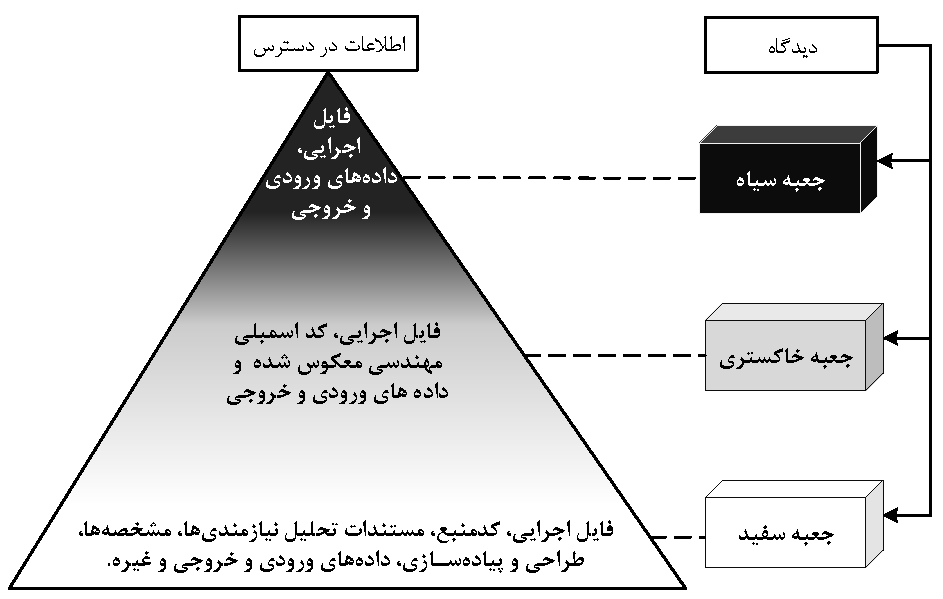
\includegraphics[width=0.75\linewidth, clip=true,  trim= 0 0 0 0]{chapter2/ch2_box_veiw_test_triangle_crop.pdf}
    \caption[ انواع روش‌های آزمون نرم‌افزار]
    {
        انواع روش‌های آزمون نرم‌افزار
    }
    \label{fig:ch2_box_veiw_test_triangle_crop}
\end{figure}

\section{درج جدول}
در اینجا نمونه‌ای از یک جدول به همراه ارجاع به آن در متن آماده است.
جدول
\ref{tabel:metrics}
متریک‌های مورد استفاده در رساله پیشنهادی را به تفکیک موضوع و سطح، نشان می‌دهد.  

\begin{table}[]
    \centering
    \caption[متریک‌های استفاده شده در رساله پیشنهادی]
    {متریک‌های نرم‌افزار
}
    \label{tabel:metrics}
    \resizebox{0.85\linewidth}{!}{%
        \begin{latin}

        \begin{tabular}{lllllll}
            \hline
            Subject     & Metric name                                      & Abbrivation & Method & Class & File & Package \\ \hline
            Size/Count  & Line of code                                     & LOC         & *      & *     & *    & *       \\
            & Number of statements                             & NOSM        & *      & *     & *    & *       \\
            & Number of static   methods                       & NOSM        &        & *     & *    & *       \\
            & Number of static   attributes                    & NOSA        &        & *     & *    & *       \\
            & Number of instance   methods                     & NOIM        &        & *     & *    & *       \\
            & Number of instance   attributes                  & NOIA        &        & *     & *    & *       \\
            & Number of method                                 & NOMT        &        & *     & *    & *       \\
            & Number of not accessor   or mutator methods      & NOMTNAMM    &        & *     & *    & *       \\
            & Number of constructores                          & NOCON       &        & *     &      &         \\
            & Number of parameters                             & NOP         & *      & *     & *    & *       \\
            & Number of classes                                & NOCS        &        &       & *    & *       \\
            & Number of files                                  & NOFL        &        &       &      & *       \\
            Complexity  & Cyclomatic complexity                            & CC          & *      & *     & *    & *       \\
            & Number of unique paths though a body of   code   & PATH        & *      & *     & *    & *       \\
            & Nesting level                                    & NESTING     & *      & *     & *    & *       \\
            & Number of overlapping jumps                      & KNOTS       & *      & *     & *    & *       \\
            Dependency  & Lack of cohesion in methods                      & LOCM        &        & *     &      &         \\
            & Coupling between   objects                       & CBO         &        & *     &      &         \\
            & Response for a class                             & RFC         &        & *     &      &         \\
            & Number of incoming invocations                   & FANIN       & *      & *     & *    & *       \\
            & Number of outgoing invocations                   & FANOUT      & *      & *     & *    & *       \\
            & Called foreign not   accessor or mutator methods & CFNAMM      &        & *     &      &         \\
            & Access to foreign data                           & ATFD        &        & *     &      &         \\
            & Data abstraction   coupling                      & DAC         &        & *     &      &         \\
            Visibility  & Number of default   methods                      & NODM        &        & *     & *    & *       \\
            & Number of private   methods                      & NOPM        &        & *     & *    & *       \\
            & Number of protected   methods                    & NOPRM       &        & *     & *    & *       \\
            & Number of public   methods                       & NOPLM       &        & *     & *    & *       \\
            & Number of accessor   methods                     & NOAM        &        & *     & *    & *       \\
            Inheritance & Depth of inheritance   tree                      & DIT         &        & *     &      &         \\
            & Number of children                               & NOC         &        & *     &      &         \\
            & Number of parents                                & NOP         &        & *     &      &         \\
            & Number of inherited   methods                    & NIM         &        & *     &      &         \\
            & Number of methods   overridden                   & NMO         &        & *     &      &         \\
            & Number of implemented interfaces                 & NOII        &        & *     &      &         \\
            Total       & 35                                               &             & 9      & 33    & 21   & 22      \\ \hline
        \end{tabular}%
        \end{latin}   
 }
\end{table}
 
 
 \section{درج الگوریتم}
 یکی از نقاط قوت 
 \LaTeX
 امکان حروف‌چینی بسیار خوانای الگوریتم‌ها و شبه‌کدها است که معمولاً در نوشتارهای مهندسی کامپیوتر وجود دارند. در اینجا یک نمونه الگوریتم (الگوریتم 
  \ref{alg:data-neural-fuzz}
 ) برای نمونه قرار داده شده است:
 
 %%% My algorithms %%%
 %%
 %% 1 - DataNeuralFuzz
 %%
 \begin{algorithm}%[ht]
     \onehalfspacing
     \caption{\lr{DataNeuralFuzz}} \label{alg:data-neural-fuzz}
     \begin{latin}
         %\begin{algorithmic}[1]
         \DontPrintSemicolon
         \setcounter{AlgoLine}{0}
         \LinesNumbered
         
         \SetKwFunction{Random}{Random}
         \SetKwFunction{RandInt}{RandInt}
         \SetKwFunction{Predict}{Predict}
         \SetKwFunction{EndsWith}{EndsWith}
         \SetKwFunction{Sample}{Sample}
         \SetKwFunction{Chars}{Chars}
         \SetKwFunction{Len}{Len}
         \SetKwFunction{AddBinaryPart}{AddBinaryPart}
         \SetKwFunction{MutateBinaryPart}{MutateBinaryPart}
         \SetKwInput{KwData}{Input}
         \SetKwInput{KwResult}{Output}
         
         \KwData{Learnt model $M$, Sequence prefix $P$, Diversity $D$, Fuzzing rate $FR$, End token $ET$, Binary token $BT$}
         \KwResult{Test data $TD$}
         
         \BlankLine
         
         $TD$  $\gets$ $P$\;
         
         $MaxLen$  $\gets$ \RandInt($a$, $b$)\;
         
         \While{$not$ \EndsWith($TD$, $ET$)}
         {
             $predicts$  $\gets$ \Predict($M$($P$))\;
             
             $c$, $p(c)$  $\gets$ \Sample($predicts$, $D$) \tcc*{Sample c from the learnt model}\;
             
             $p\_fuzz$  $\gets$ \Random($0,1$) \tcc*{Decide whether to fuzz}\;
             
             \If{ $p\_fuzz<FR \wedge p(c)<\alpha \wedge c\not\in$ \Chars($BT$) $\wedge c\not\in$ \Chars($ET$)}
             {
                 $c$  $\gets$ $argmin_{c'}\{ p(c') \in predicts \}$ \tcc*{Fuzz c by c' where c' is the lowest likelihood}\;
             } 
             
             $TD$  $\gets$ $TD$ + $c$\;
             
             $P$  $\gets$ $P[1:]$ + $c$ \tcc*{Propagate fuzz to prefix and next generated data}\;
             
             \If{ \Len($TD$) > $MaxLen$ }
             {
                 $TD$  $\gets$ $TD$ + $ET$ \;
                 
                 \textbf{Break}\;
             }
             
         }
         
         \If {$BT \in TD$}
         {
             $TD$ $\gets$ \AddBinaryPart($TD$)\;
             
             $TD$ $\gets$ \MutateBinaryPart($TD$)\;
         }
         
         \textbf{Return} $TD$\;
         
         %\end{algorithmic}
     \end{latin}
 \end{algorithm}
 
 
 \section{درج فرمول‌ها و روابط ریاضی}
 برای نمونه به رابطه محاسبه سرگشتگی عنایت فرمایید. همان‌طور که مشاهده می‌شود فرمول‌ها و روابط ریاضی به‌صورت خودکار شماره‌گذاری می‌شوند.
 
  \begin{equation}\label{ppl}
     \begin{split}
         PP_{LM}(x) & = \sqrt[n]{\prod_{i=1}^n(\frac{1}{p(x^{(i)}|<x^{(1)}, ..., x^{(i-1)}>)}} \\
         & = 2^{-\frac{1}{n}\sum_{i=1}^n\log_{2}{p(x^{(i)}|<x^{(1)}, ..., x^{(i-1)>})}}
     \end{split}
 \end{equation}
 
 
 
 \section{خلاصه}
 ‌در بخش خلاصه یا نتیجه‌گیری انتهایی هر فصل، خلاصه و جمع‌بندی مطالب آن فصل ارائه می‌گردد. 
 
 